\section{An initial overview of of the course}
\title[Initial overview]{Power Electronics Devices and Components}
 
\begin{frame}[plain]
    \titlepage
\end{frame}
%%%%%%%%%%%%%%%%%%%%%%%%%%%%%%%%%%%%%%%%%%%%%%%%%%%%%%%%%%%%%
%% Overview of the course %%
%%%%%%%%%%%%%%%%%%%%%%%%%%%%%%%%%%%%%%%%%%%%%%%%%%%%%%%%%%%%%
\begin{frame}
	\frametitle{Course Overview}
The course will be in 6 modules.
		\begin{itemize}
		  \item Module I: Basics of Electronics Devices.
		  \item Module II: Towards Power Semiconductor Devices- Introduction.
		  \item Module III: Conventional Power Semiconductor Devices.
		  \item Module IV: Next Generation Power Semiconductor Devices.
		  \item Module V: Passive Components.
		  \item Module VI: Way forward- Power Modules, Reliability, and Thermal Management
		\end{itemize}
\textbf{Pattern of class}: \\ Day: Thursday, every week \\ 
Time: 4 pm to 6 pm (theory) and 6 pm to 8 pm (tutorial) (ideally but it can change) \\
Holidays: 1st May, 29 May, and 19 June 2025. As required classes will be rescheduled. 
\end{frame}

%%%%%%%%%%%%%%%%%%%%%%%%%%%%%%%%%%%%%%%%%%%%%%%%%%%%%%%%%%%%%
%% Teaching Support Team %%
%%%%%%%%%%%%%%%%%%%%%%%%%%%%%%%%%%%%%%%%%%%%%%%%%%%%%%%%%%%%%
\begin{frame}
	\frametitle{The teaching team}
	\vspace{-0.5cm}
	\begin{columns}[t]
\centering
		\column[T]{0.5\textwidth}
		\begin{figure}
			\centering
				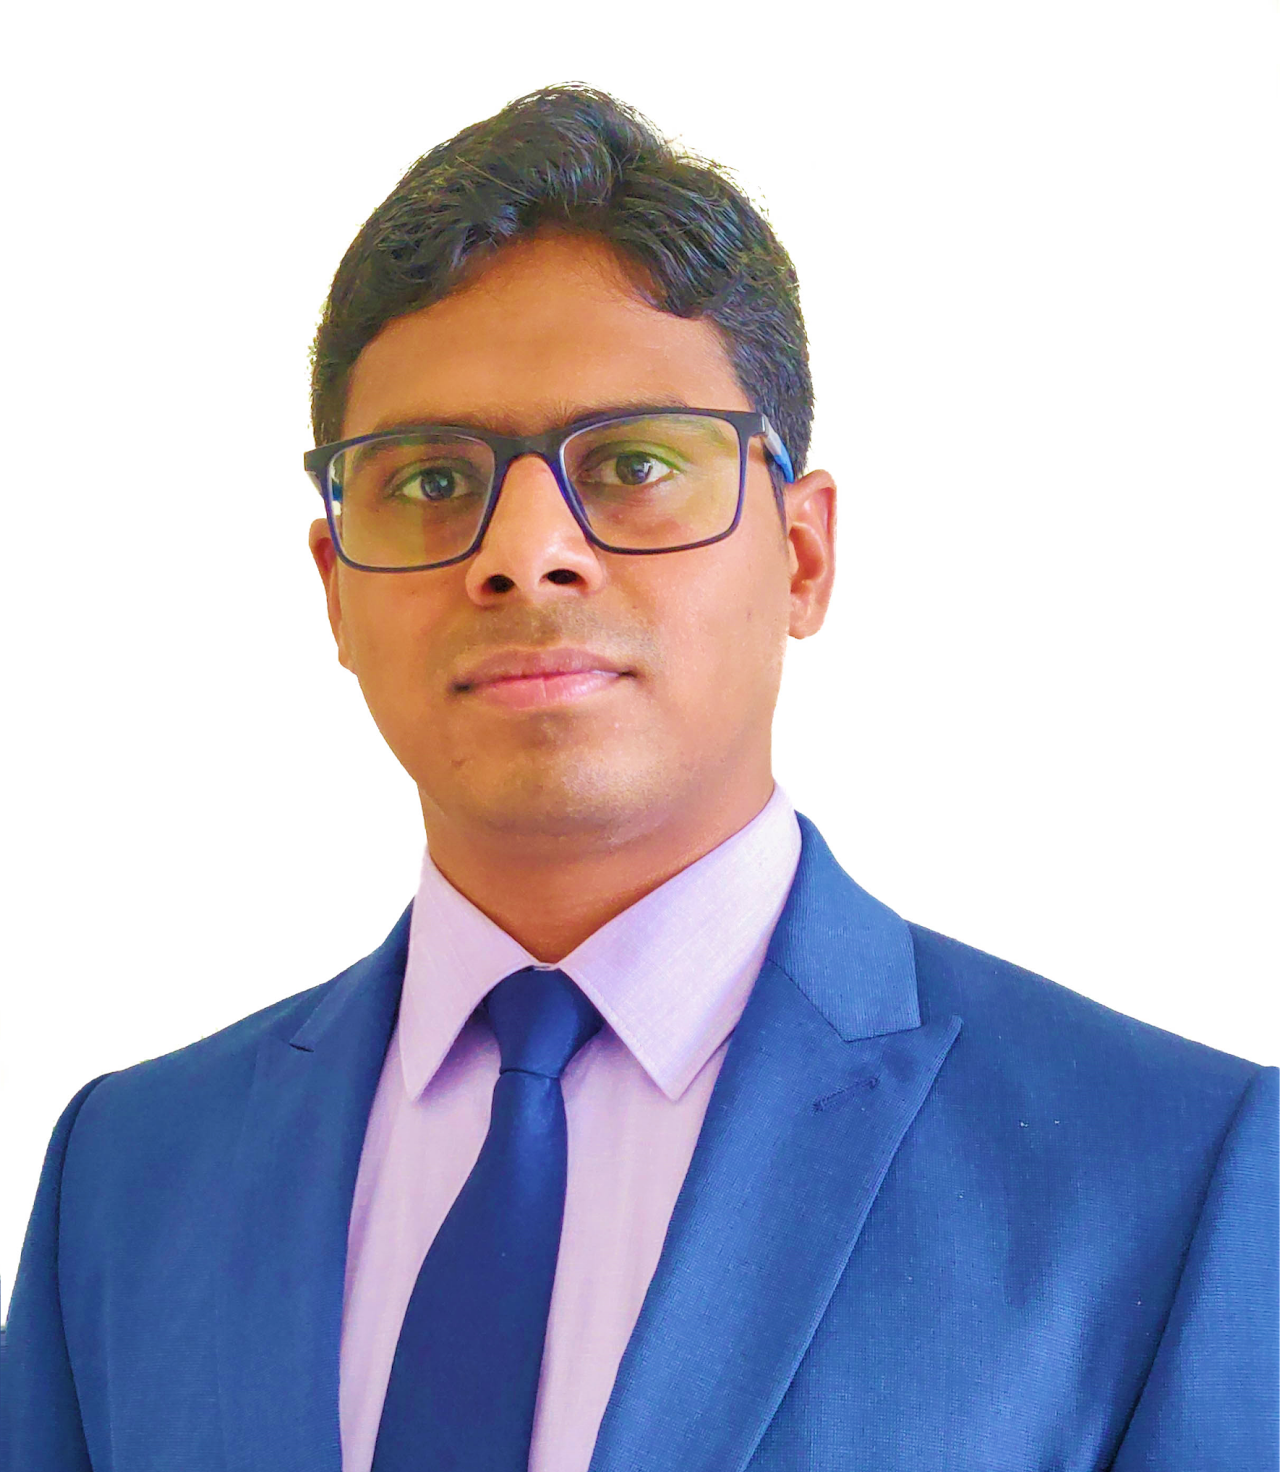
\includegraphics[height=2.5cm]{fig/lec01/Bikash.png}
				\caption*{Bikash Sah}
		\end{figure}
	
		\column[T]{0.5\textwidth}
		\begin{figure}
			\centering
				\includegraphics[height=2.5cm]{fig/lec01/ASack.jpg}
				\caption*{Andreas Sack}
		\end{figure}		
	\end{columns}
	\vspace{-0.5cm}
	\begin{varblock}{Contact}
		\begin{itemize}
			\item Email: see \href{https://www.eti.uni-siegen.de/ias/}{chair's homepage}
			\item Offices: H-A building, 4th floor
			\item Individual appointments on request (remote or personally)
            \item Multiple relevant courses are offered by the Chair.  \href{https://www.eti.uni-siegen.de/ias/teaching/}{Check link!}
		\end{itemize}
	\end{varblock}
** \small{Future follow-up courses are planned to be introduced in next semester- High Frequency Power Electronics, etc.}
	\end{frame}



%%%%%%%%%%%%%%%%%%%%%%%%%%%%%%%%%%%%%%%%%%%%%%%%%%%%%%%%%%%%%
%% Start %%
%%%%%%%%%%%%%%%%%%%%%%%%%%%%%%%%%%%%%%%%%%%%%%%%%%%%%%%%%%%%%
\begin{frame}
\center
\textbf{\huge{Module I: Basics of Electronics Devices}}
\end{frame}

%%%%%%%%%%%%%%%%%%%%%%%%%%%%%%%%%%%%%%%%%%%%%%%%%%%%%%%%%%%%%
%% What is Electronics %%
%%%%%%%%%%%%%%%%%%%%%%%%%%%%%%%%%%%%%%%%%%%%%%%%%%%%%%%%%%%%%
\begin{frame}
	\frametitle{What are "Electronic Devices"?}
	\begin{columns}
		\begin{column}{0.5\textwidth}
			\begin{varblock}{Electronic Devices}
				Electronic devices are hardware components which leverage the property of materials to control the flow of electrons or charge.
			\end{varblock} \vspace{-0.5cm}		
			\begin{itemize}
				\item<2-> Have a long history of development- started with the invention of vaccum tube or Thermionic valve in 1904 by J.A. Fleming.
				\item<3-> The first transistor was invented in 1947 by J.Bardeen, W.H. Brattain and W.S. Shockley in Bell Labs.
				\item<4-> The first integrated circuit was invented in 1958 by J. Kilby and R. Noyce -- On and it goes
%				\item<5-> The first microprocessor was invented in 1971 by F. Faggin, T. Klein and H. Hoff in Intel.
%				\item<6-> The first microcontroller was invented in 1971 by F. Faggin, T. Klein and H. Hoff in Intel.
%				\item<7-> On and it goes- every day new devices are invented and developed.
			\end{itemize}
		\end{column}
		\begin{column}{0.5\textwidth}
			\begin{figure}
				\centering
				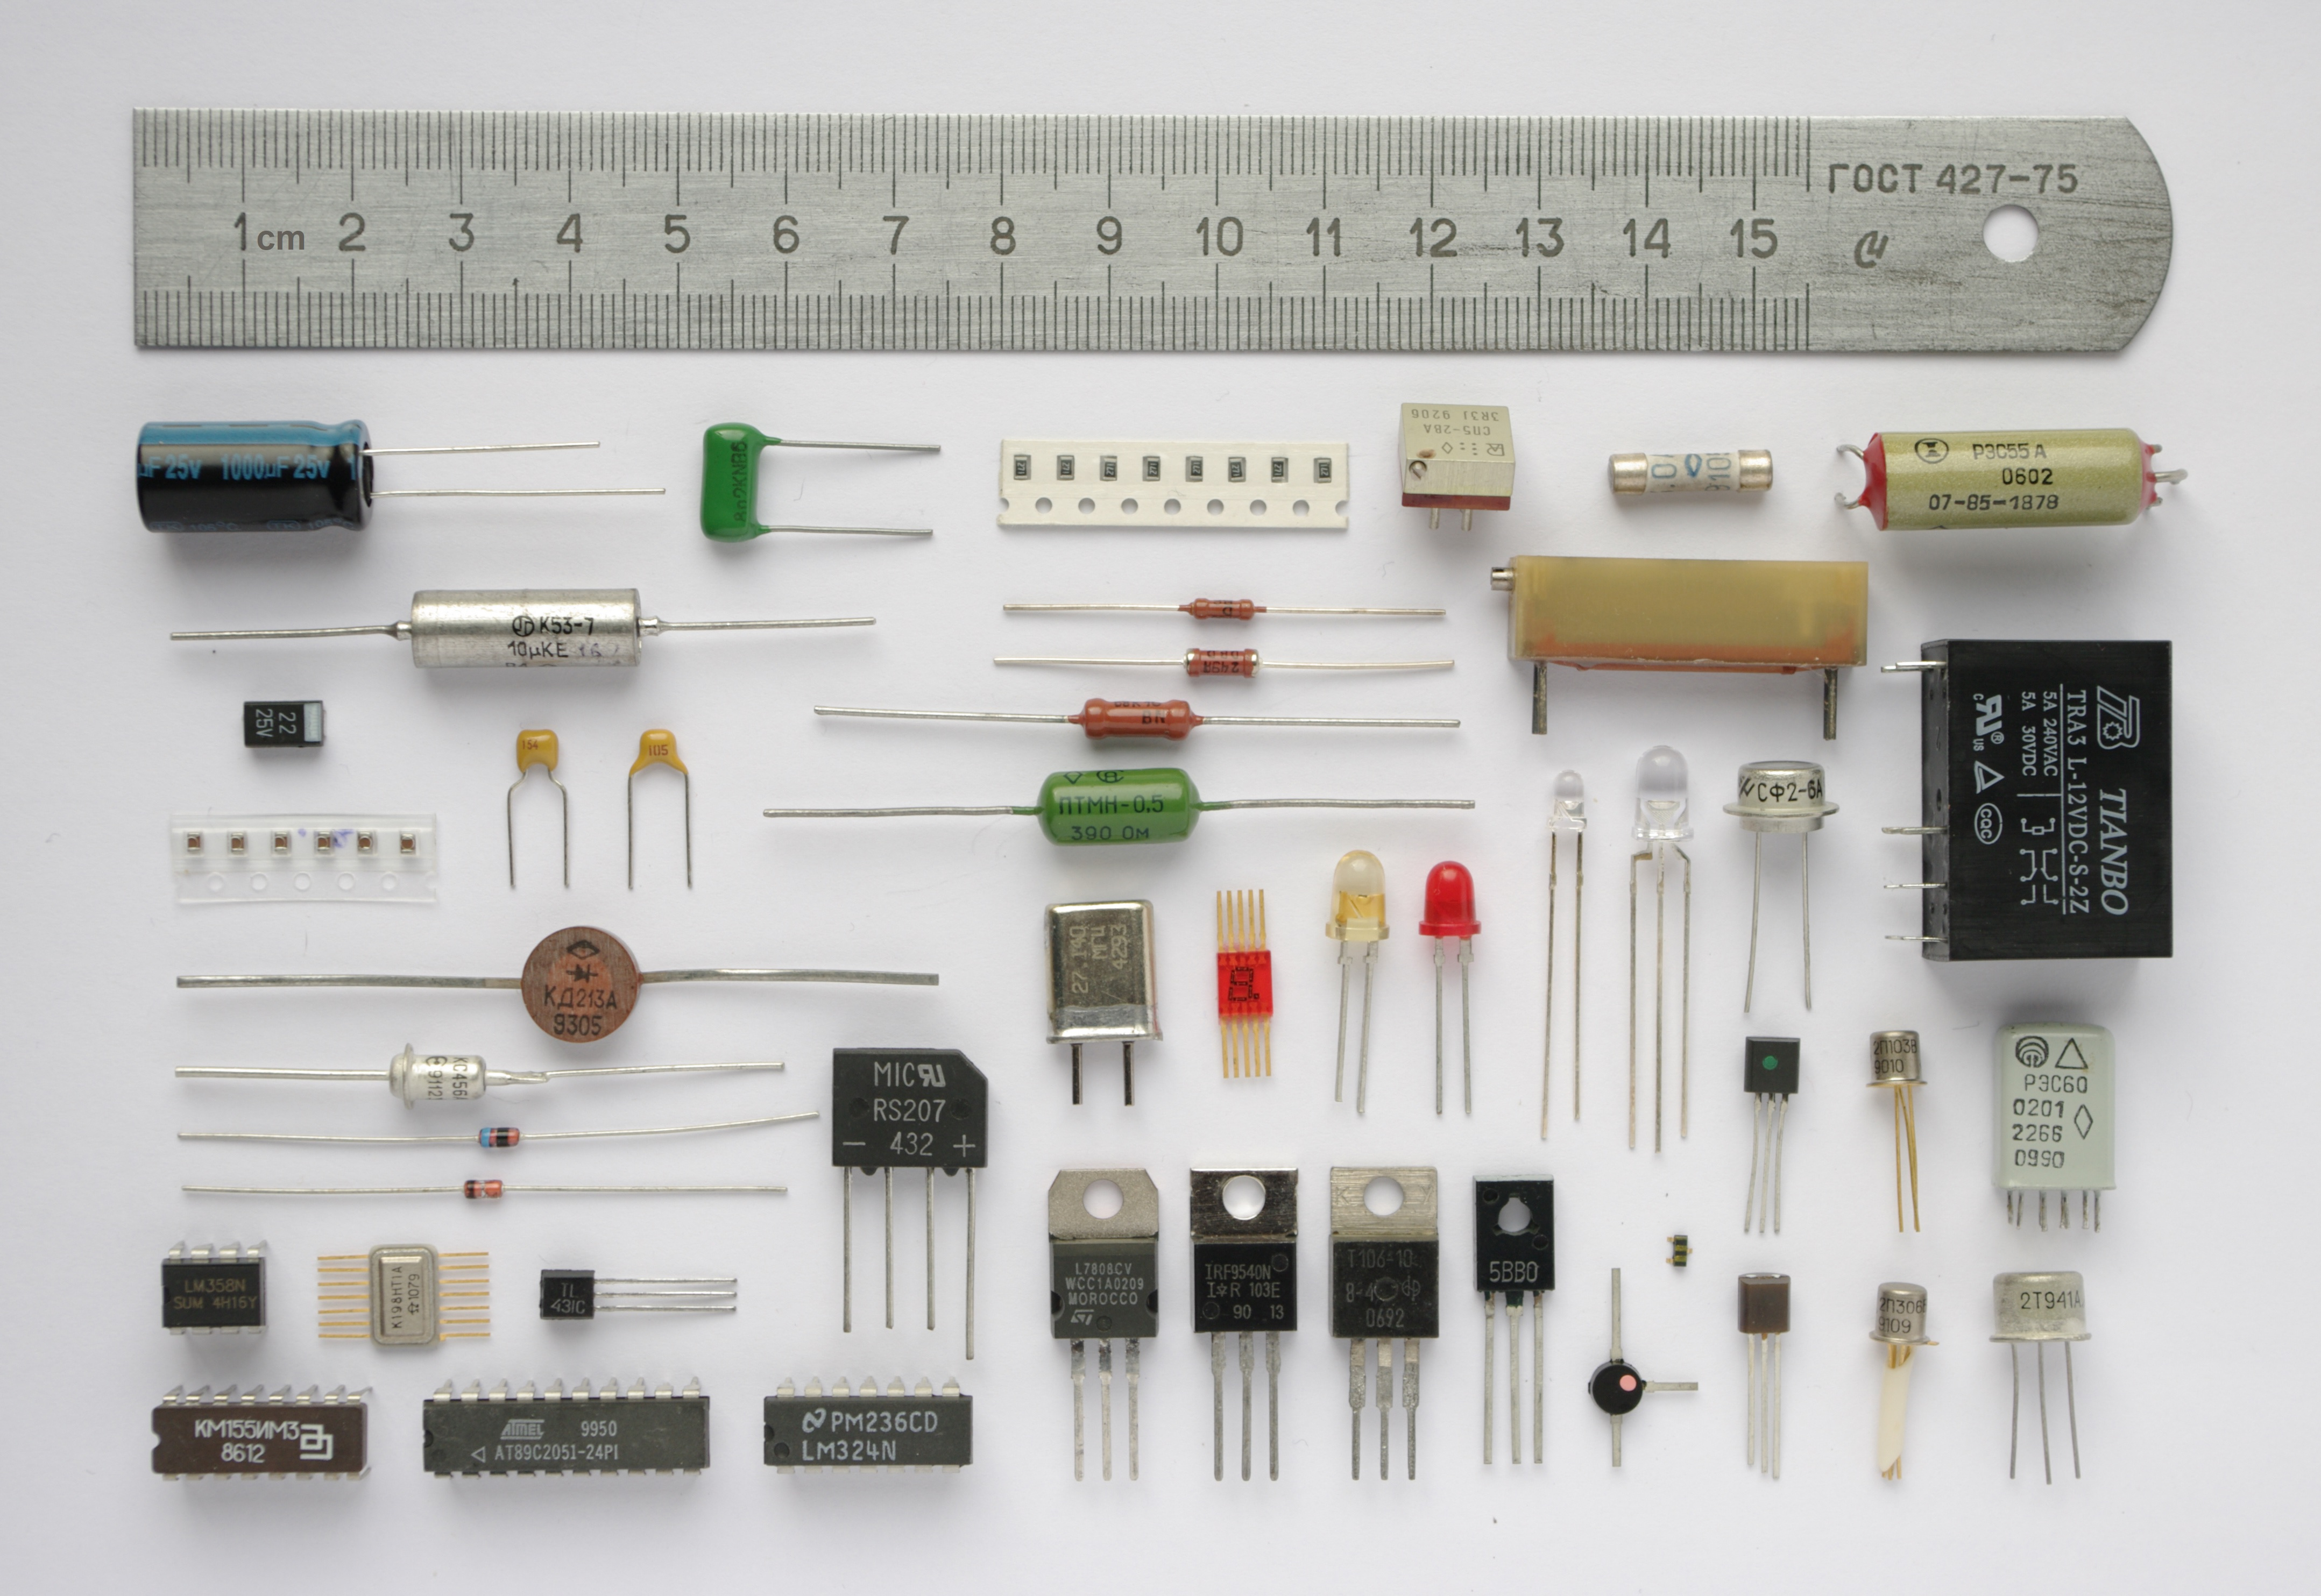
\includegraphics[scale= 0.05]{fig/lec01/Componentes.jpg}
				\caption{Example of electronic components (source: \href{https://commons.wikimedia.org/wiki/File:Componentes.JPG}{Wikimedia Commons}, Kae, public domain)}
			\end{figure}
		\end{column}
		\end{columns}
\end{frame}

%%%%%%%%%%%%%%%%%%%%%%%%%%%%%%%%%%%%%%%%%%%%%%%%%%%%%%%%%%%%%
%% Classification of electronics? %%
%%%%%%%%%%%%%%%%%%%%%%%%%%%%%%%%%%%%%%%%%%%%%%%%%%%%%%%%%%%%%
\begin{frame}
	\frametitle{General classification of "Electronic Devices"?}
	\begin{columns}
		\begin{column}{0.5\textwidth}

			\begin{itemize}
				\item<2-> Active devices: These are the devices which can control the flow of current and mainly consists of \textbf{semiconductor} materials. Examples: Transistor, Diode, etc.
				\item<3-> Passive devices: These are the devices which cannot control the flow of current and perform operation lke consuming, storing, or releasing power. Examples: Resistor, Capacitor, Inductor, etc.
			\end{itemize}
		\end{column}
		\begin{column}{0.5\textwidth}
			\begin{figure}
				\centering
				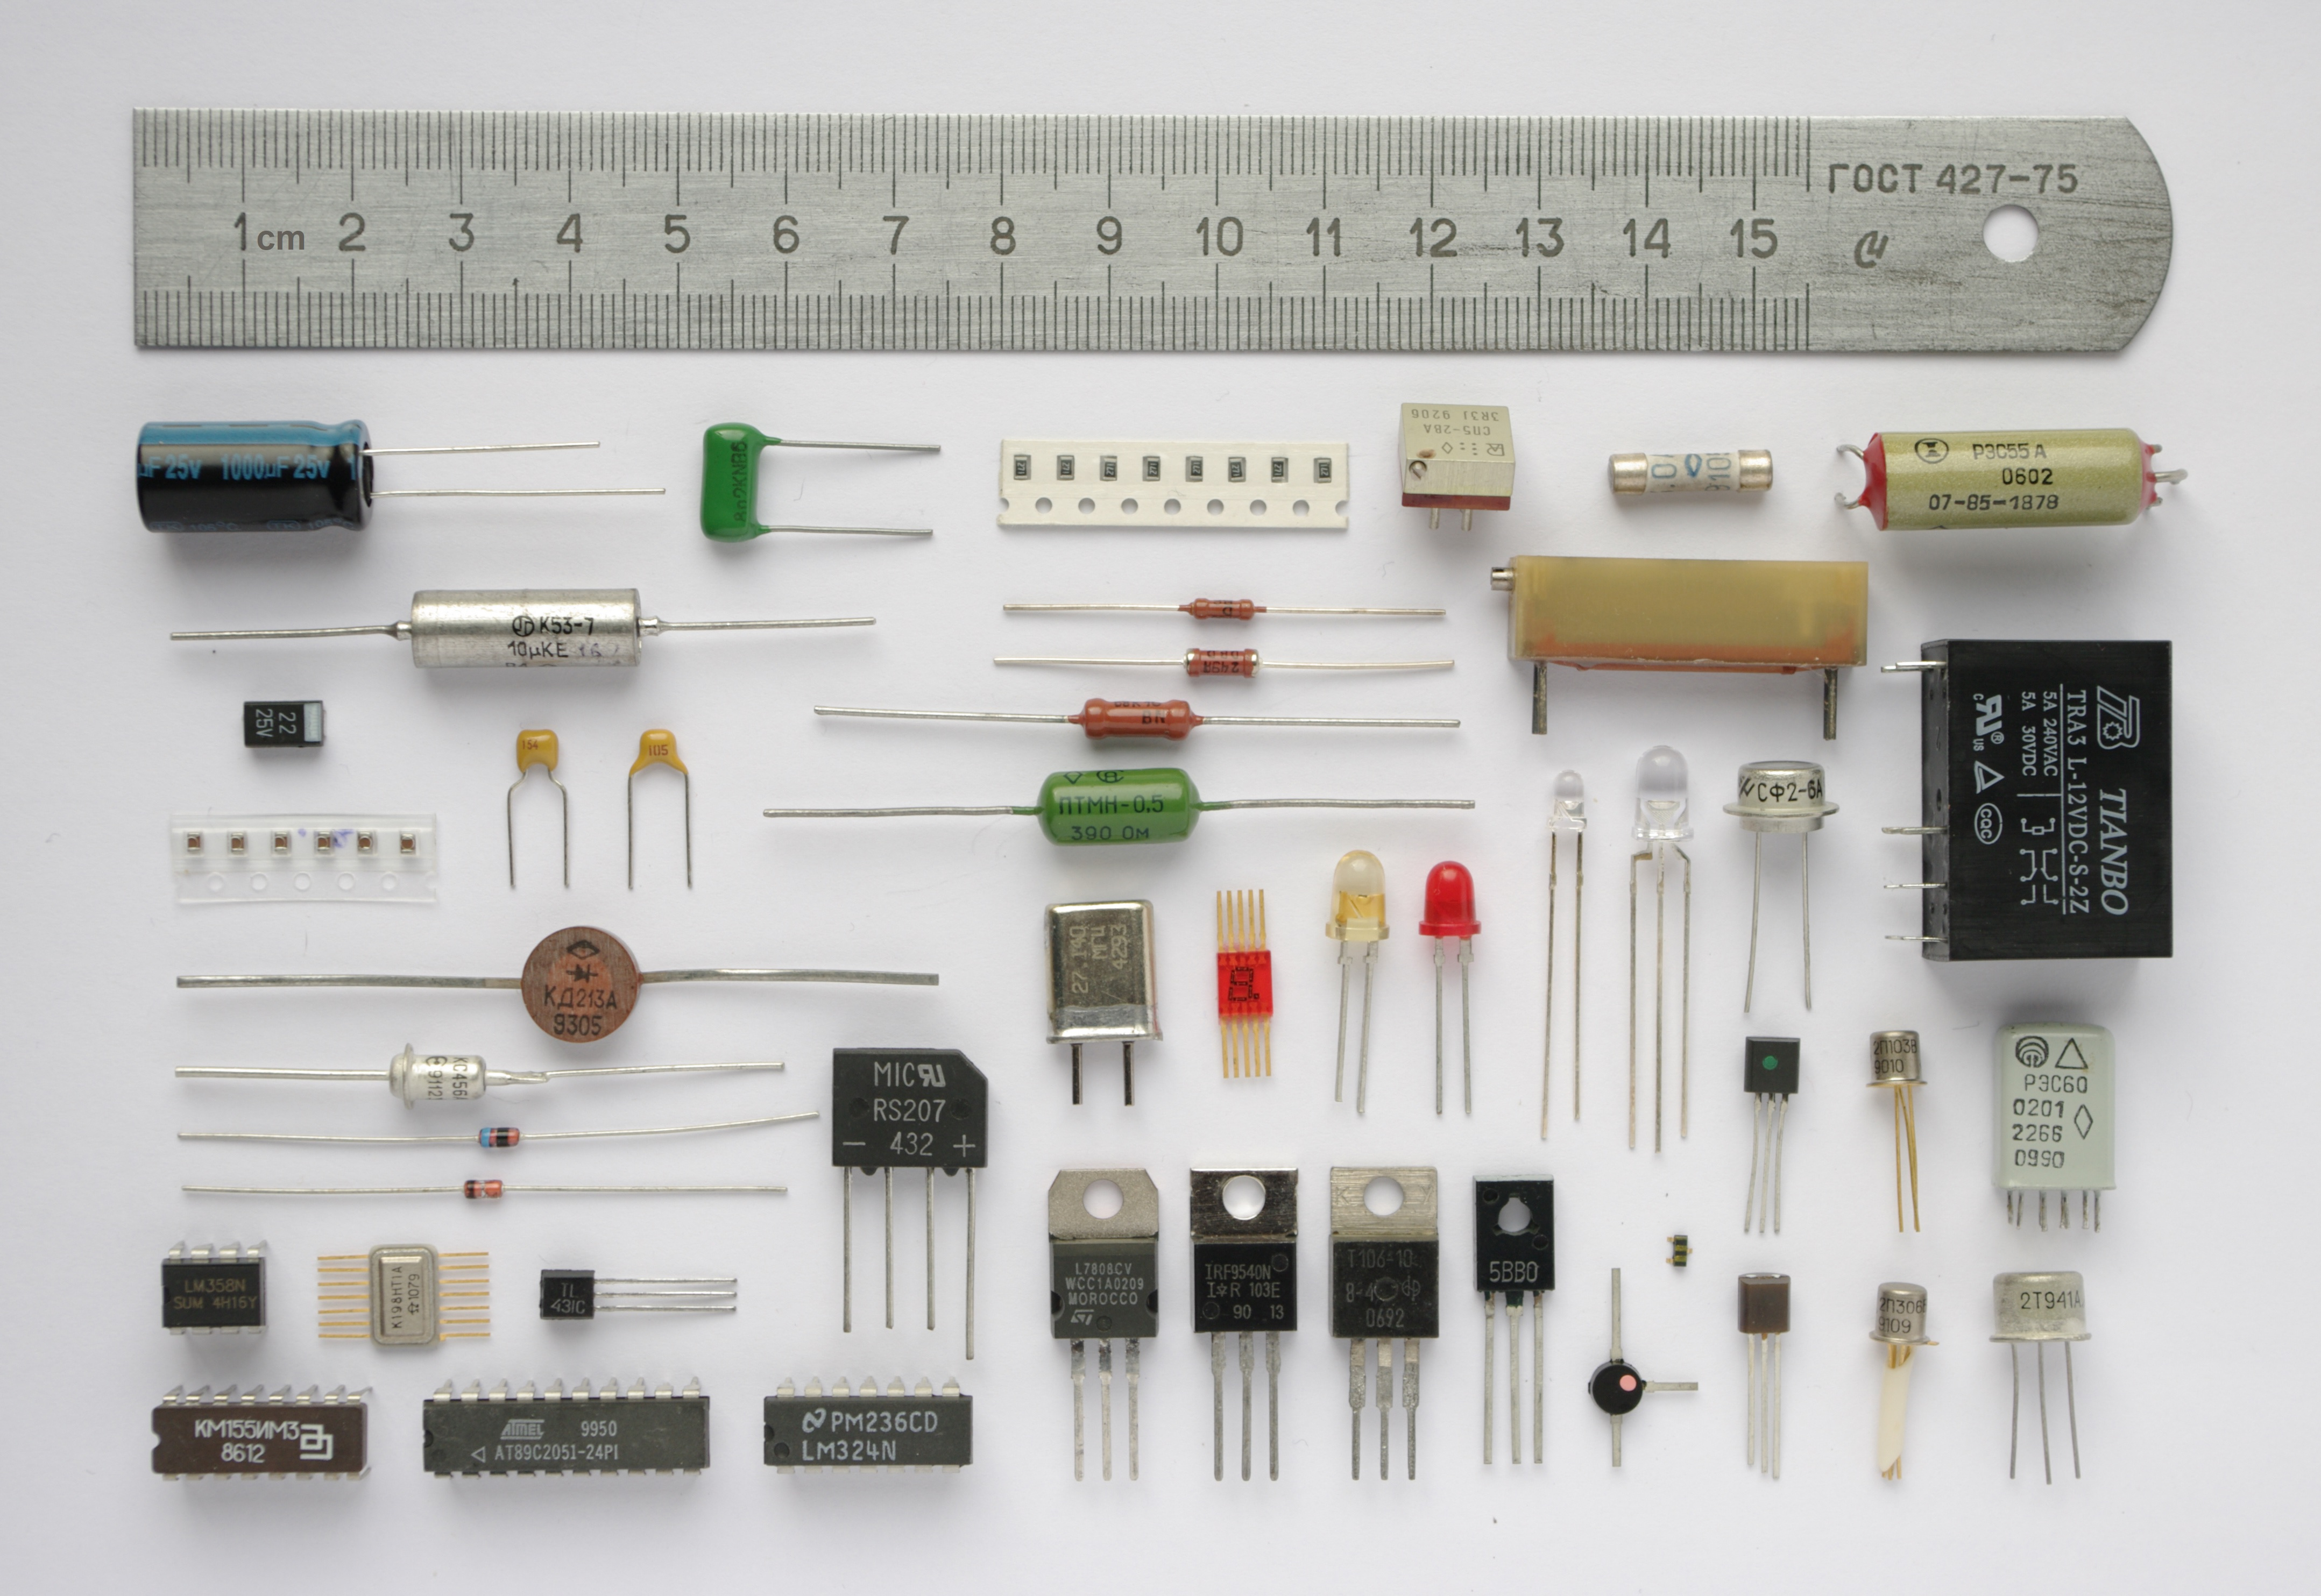
\includegraphics[scale= 0.05]{fig/lec01/Componentes.jpg}
				\caption{Example of electronic components (source: \href{https://commons.wikimedia.org/wiki/File:Componentes.JPG}{Wikimedia Commons}, Kae, public domain)}
			\end{figure}
		\end{column}
		\end{columns}
\end{frame}

%%%%%%%%%%%%%%%%%%%%%%%%%%%%%%%%%%%%%%%%%%%%%%%%%%%%%%%%%%%%%
%% Towards power electronics- difference between electroics and power electronics %%
%%%%%%%%%%%%%%%%%%%%%%%%%%%%%%%%%%%%%%%%%%%%%%%%%%%%%%%%%%%%%
\begin{frame}
	\frametitle{Comparison of Electronics and Power Electronics}
	\begin{table}[htbp] \small
		\centering
		\caption{Comparison between Electronics and Power Electronics} \footnotesize
		\begin{tabular}{|p{2.5cm}|p{4cm}|p{5cm}|}
		\hline
		\textbf{Feature} & \textbf{Electronics} & \textbf{Power Electronics} \\
		\hline
		\textbf{Primary Focus} & Signal processing, computation, communication & Energy conversion, control, and delivery \\
		\hline
		\textbf{Power Levels} & $\mu$W to a few watts & Tens of watts to megawatts \\
		\hline
		\textbf{Speed} & High-speed logic, RF, GHz range & Lower switching frequency (kHz–MHz), but high voltage/current \\
		\hline
		\textbf{Core Devices} & BJTs, MOSFETs, ICs, Op-Amps, Logic Gates & Diodes, IGBTs, Power MOSFETs, SCRs, SiC/GaN devices \\
		\hline
		\textbf{Applications} & Microprocessors, audio amps, sensors, mobile phones & EVs, solar inverters, motor drives, HVDC systems \\
		\hline
		\textbf{Design Challenges} & Noise, bandwidth, gain, low power & Efficiency, thermal stress, EMI, ruggedness \\
		\hline
		\textbf{Energy Handling} & Information carriers (signals) & Bulk power carriers (watts, kilowatts, megawatts) \\
		\hline
		\end{tabular}
		\end{table}
\end{frame}

%%%%%%%%%%%%%%%%%%%%%%%%%%%%%%%%%%%%%%%%%%%%%%%%%%%%%%%%%%%%%
%% Where do you find active and passive components %%
%%%%%%%%%%%%%%%%%%%%%%%%%%%%%%%%%%%%%%%%%%%%%%%%%%%%%%%%%%%%%
\begin{frame}
	\frametitle{Locating active and passive components in real world}
	\begin{figure}
		\centering
		\begin{subfigure}[t]{0.4\textwidth}
			\centering
			\includegraphics[scale=0.4]{fig/lec01/Charger_1.jpg}
			\caption{Example charging station (source: \href{https://commons.wikimedia.org/wiki/File:Nissan_LEAF_got_thirsty.jpg}{Wikimedia Commons}, \href{https://creativecommons.org/licenses/by-sa/3.0/deed.en}{CC BY 2.0})}
		\end{subfigure}
		%\hfill
		\begin{subfigure}[t]{0.4\textwidth}
			\centering
			\includegraphics[scale=0.175]{fig/lec01/charger_2.jpg}
			\caption{Public mobile charging machine (source: \href{https://commons.wikimedia.org/wiki/File:CellPhoneChargingStation.jpg}{Wikimedia Commons}, Raysonho, \href{https://creativecommons.org/publicdomain/zero/1.0/deed.ru}{CC0 1.0})}
		\end{subfigure}
	\end{figure}
\end{frame}


%%%%%%%%%%%%%%%%%%%%%%%%%%%%%%%%%%%%%%%%%%%%%%%%%%%%%%%%%%%%%
%% Where do you find active and passive components %%
%%%%%%%%%%%%%%%%%%%%%%%%%%%%%%%%%%%%%%%%%%%%%%%%%%%%%%%%%%%%%
\begin{frame}
	\frametitle{Locating active and passive components in real world}
	\begin{figure}
		\centering
		%\hfill
		\begin{subfigure}[t]{0.4\textwidth}
			\centering
			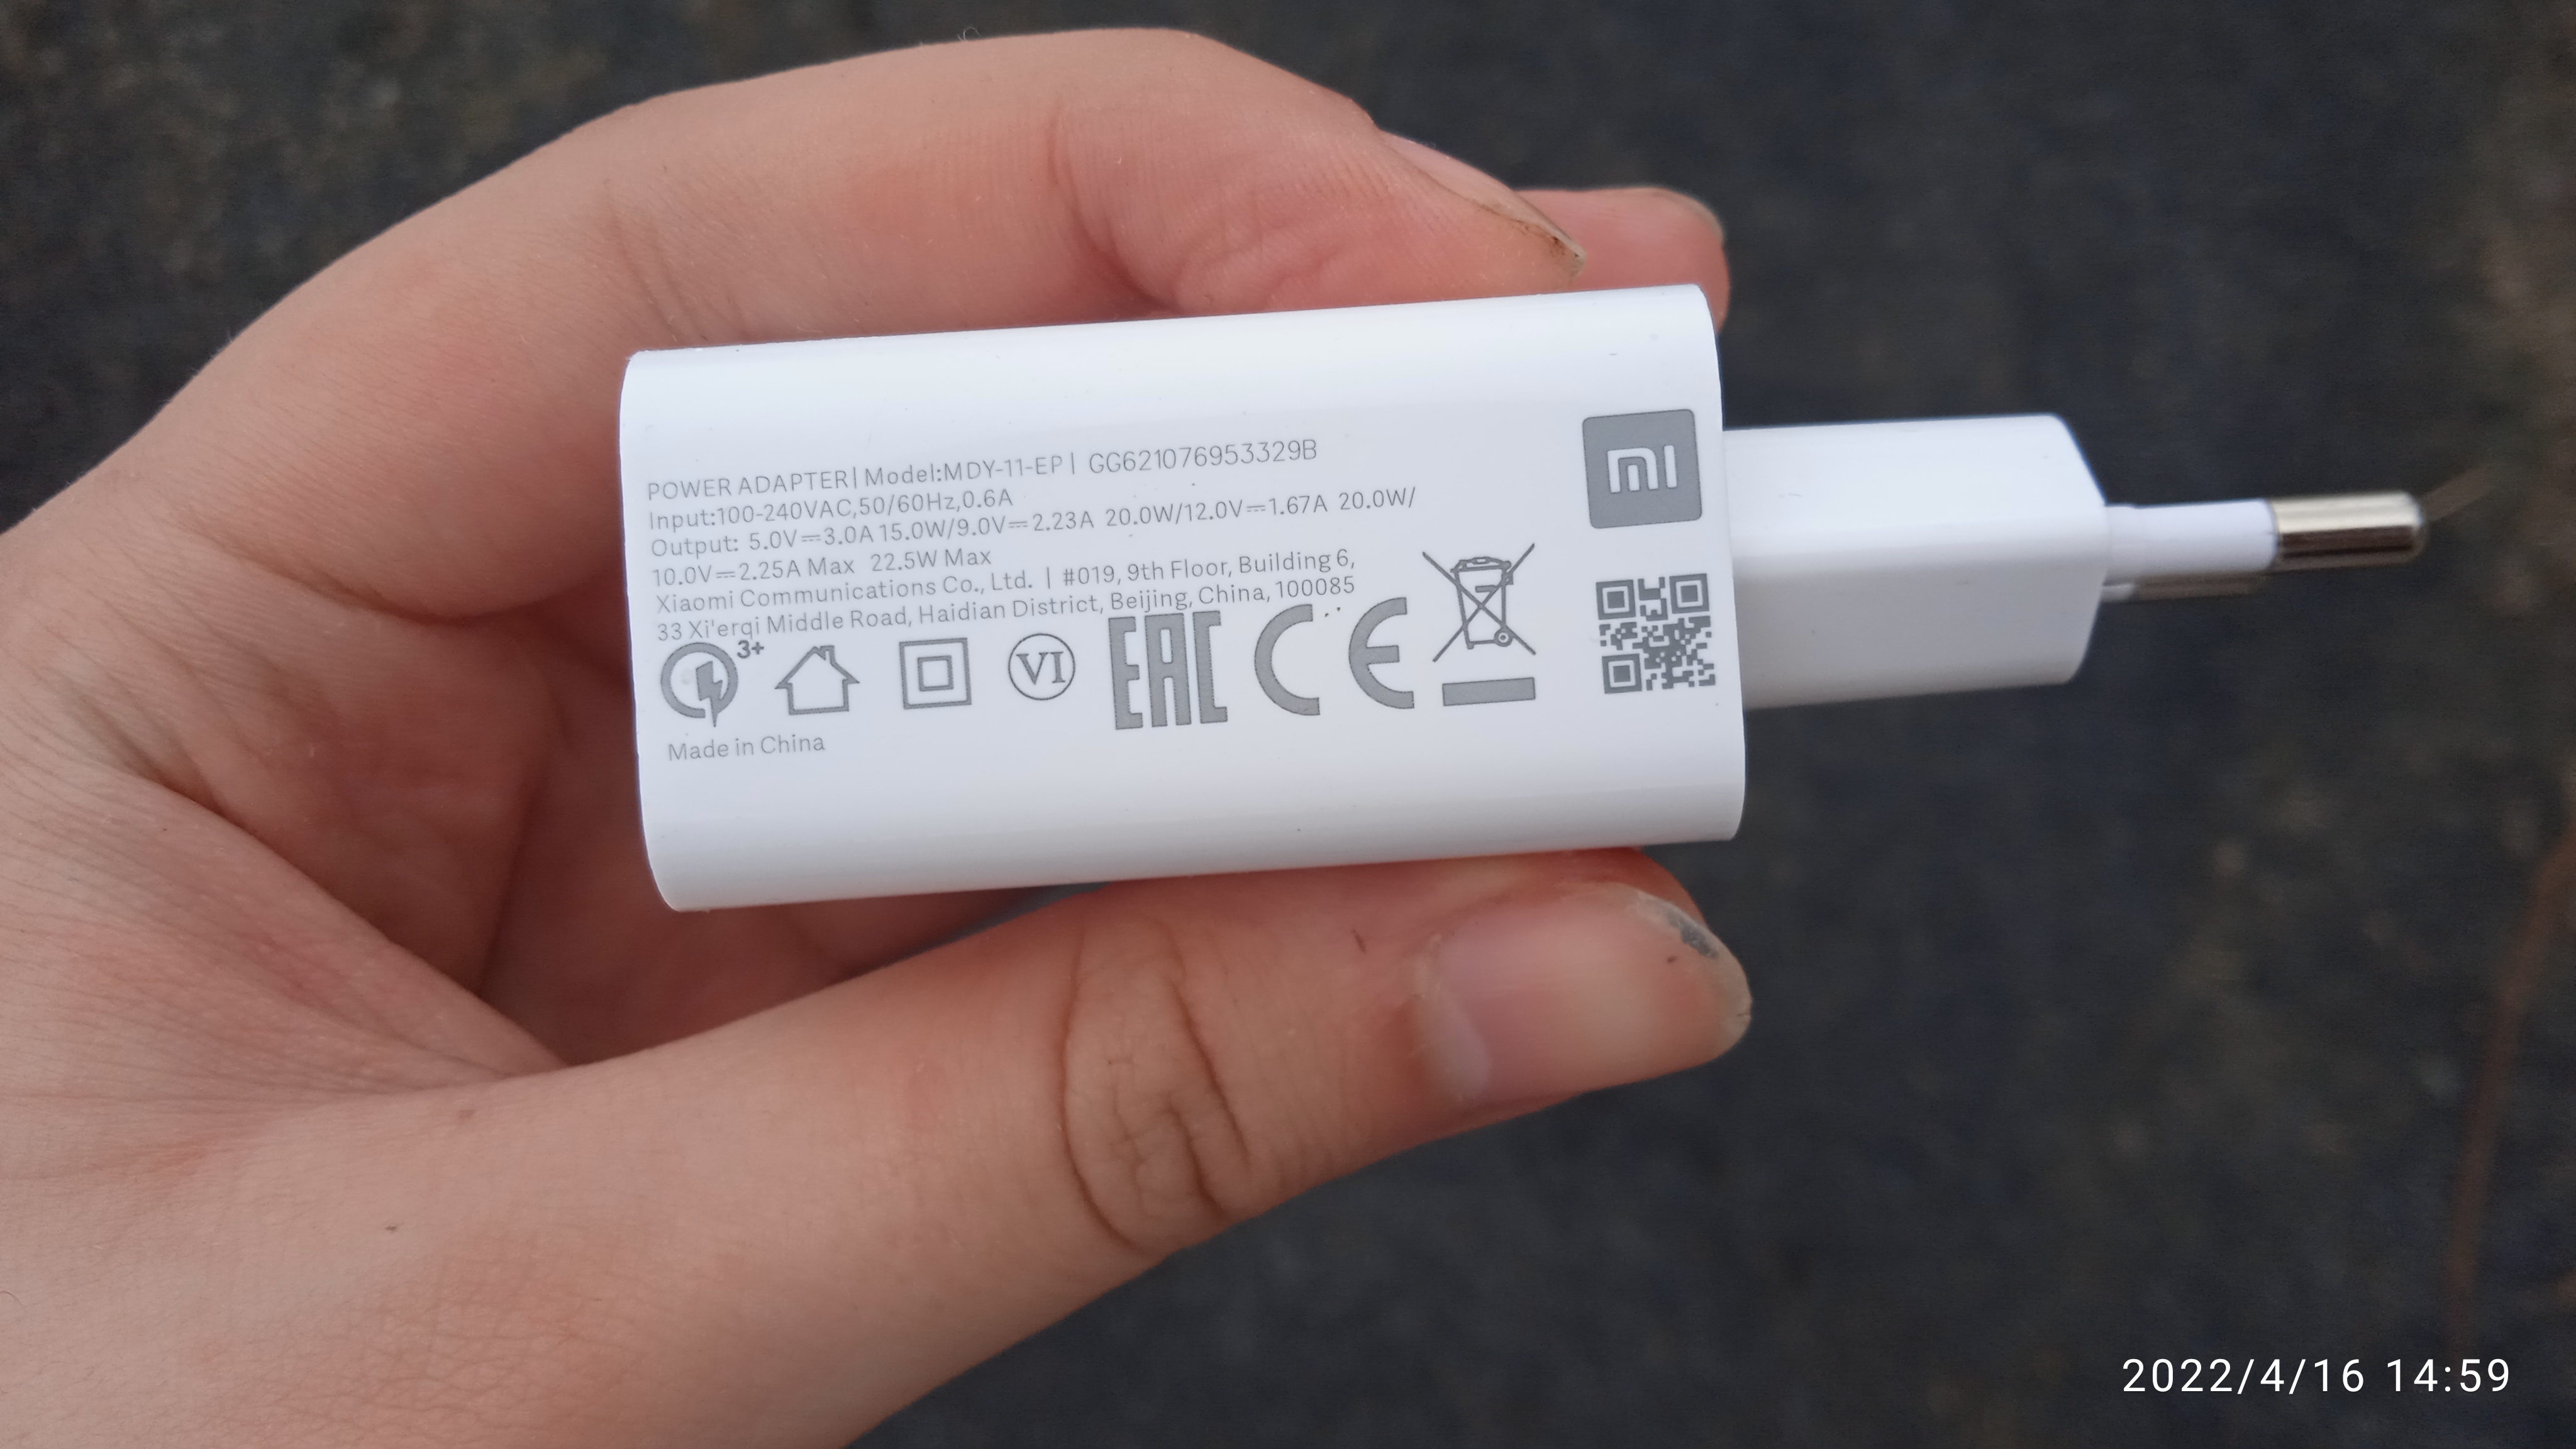
\includegraphics[scale=0.035]{fig/lec01/charger_3.jpg}
			\caption{Generic mobile phone charger (source: \href{https://commons.wikimedia.org/wiki/File:Charger_Xioami.jpg}{Wikimedia Commons}, Radio Mayak Pervouralsk, \href{https://creativecommons.org/licenses/by-sa/4.0/}{CC BY-SA 4.0})}
		\end{subfigure}
		\begin{subfigure}[t]{0.4\textwidth}
			\centering
			\includegraphics[scale=0.15]{fig/lec01/EV.jpg}
			\caption{Example electric vehicle (source: \href{https://commons.wikimedia.org/wiki/File:IBMTorontoSoftwareLabEVChargers4.jpg}{Wikimedia Commons}, Raysonho \href{https://creativecommons.org/publicdomain/zero/1.0/deed.en}{CCo 1.0})}
		\end{subfigure}
	\end{figure}
\end{frame}

%%%%%%%%%%%%%%%%%%%%%%%%%%%%%%%%%%%%%%%%%%%%%%%%%%%%%%%%%%%%%
%% Where do you find active and passive components %%
%%%%%%%%%%%%%%%%%%%%%%%%%%%%%%%%%%%%%%%%%%%%%%%%%%%%%%%%%%%%%
\begin{frame}
	\frametitle{Locating active and passive components in real world}
	\begin{figure}
		\centering
		%\hfill
		\begin{subfigure}[t]{0.4\textwidth}
			\centering
			\includegraphics[scale=0.035]{fig/lec01/wind_turbine.jpg}
			\caption{Thorntonbank Wind Farm, using 5 MW turbines REpower 5M in the North Sea off the coast of Belgium (source: \href{https://en.wikipedia.org/wiki/File:Windmills_D1-D4_(Thornton_Bank).jpg}{Wikimedia Commons}, © Hans Hillewaert, \href{https://creativecommons.org/licenses/by-sa/4.0/}{CC BY-SA 4.0})}
		\end{subfigure}
		\begin{subfigure}[t]{0.4\textwidth}
			\centering
			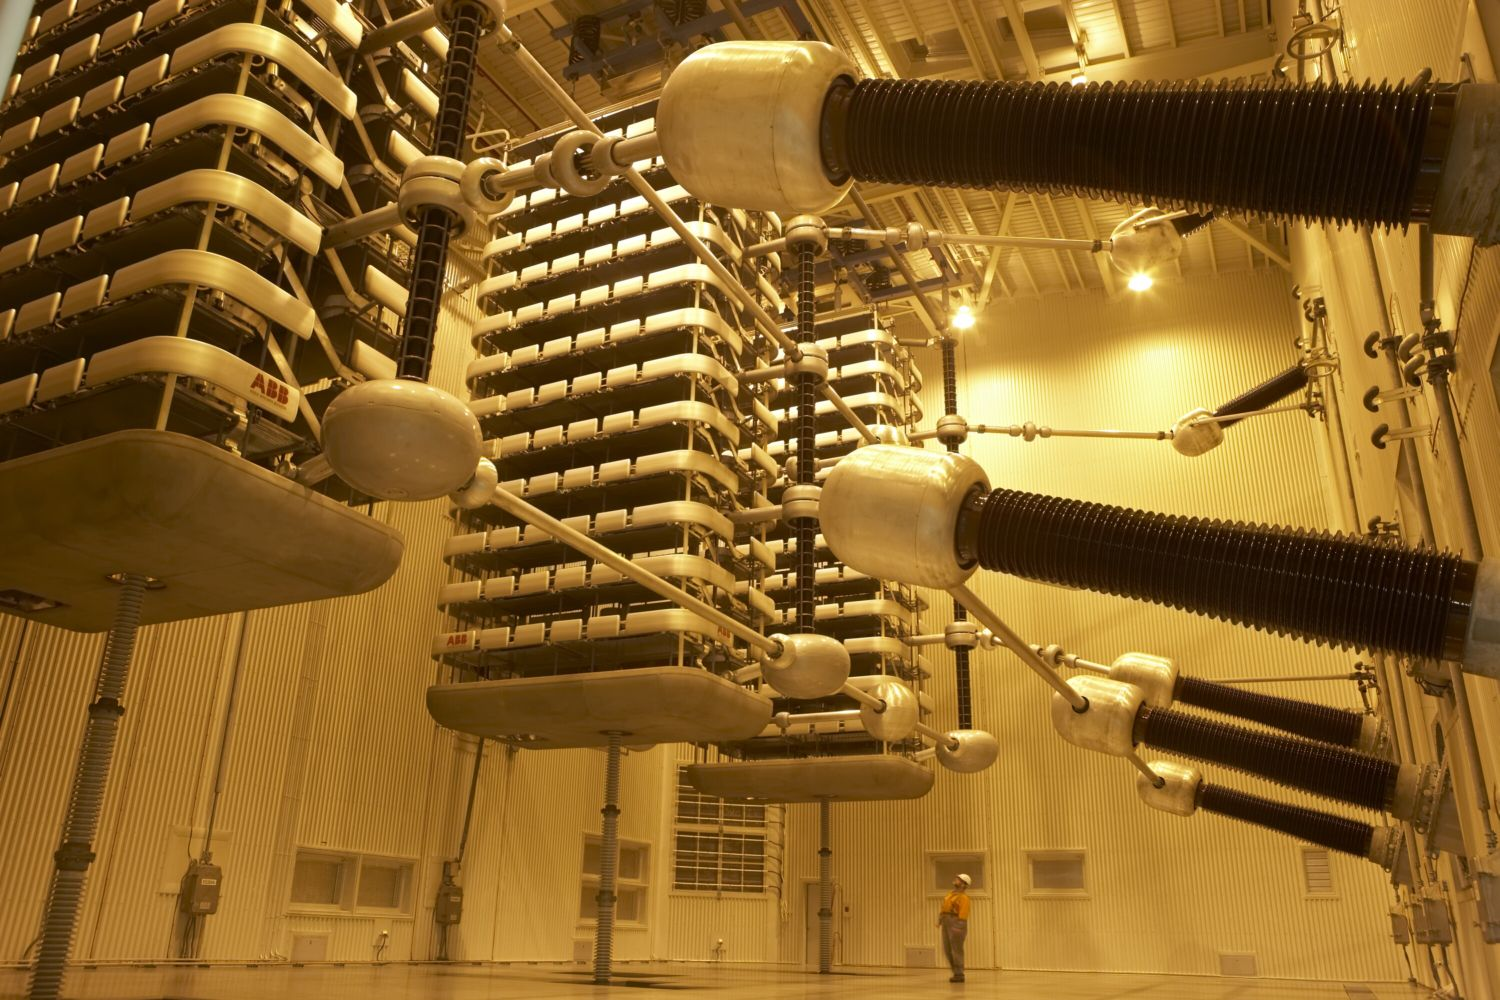
\includegraphics[scale=0.5]{fig/lec01/Thyristor.jpg}
			\caption{Thyristor valve in an HVDC (source: \href{https://commons.wikimedia.org/wiki/File:Pole_2_Thyristor_Valve.jpg}{Wikimedia Commons}, Marshelec, \href{https://creativecommons.org/licenses/by-sa/3.0}{CC BY-SA 3.0})}
		\end{subfigure}
	\end{figure}
\end{frame}

%%%%%%%%%%%%%%%%%%%%%%%%%%%%%%%%%%%%%%%%%%%%%%%%%%%%%%%%%%%%%
%% Where do you find active and passive components %%
%%%%%%%%%%%%%%%%%%%%%%%%%%%%%%%%%%%%%%%%%%%%%%%%%%%%%%%%%%%%%
\begin{frame}
	\frametitle{Locating active and passive components in real world}
	\begin{figure}
		\centering
		%\hfill
		\begin{subfigure}[t]{0.4\textwidth}
			\centering
			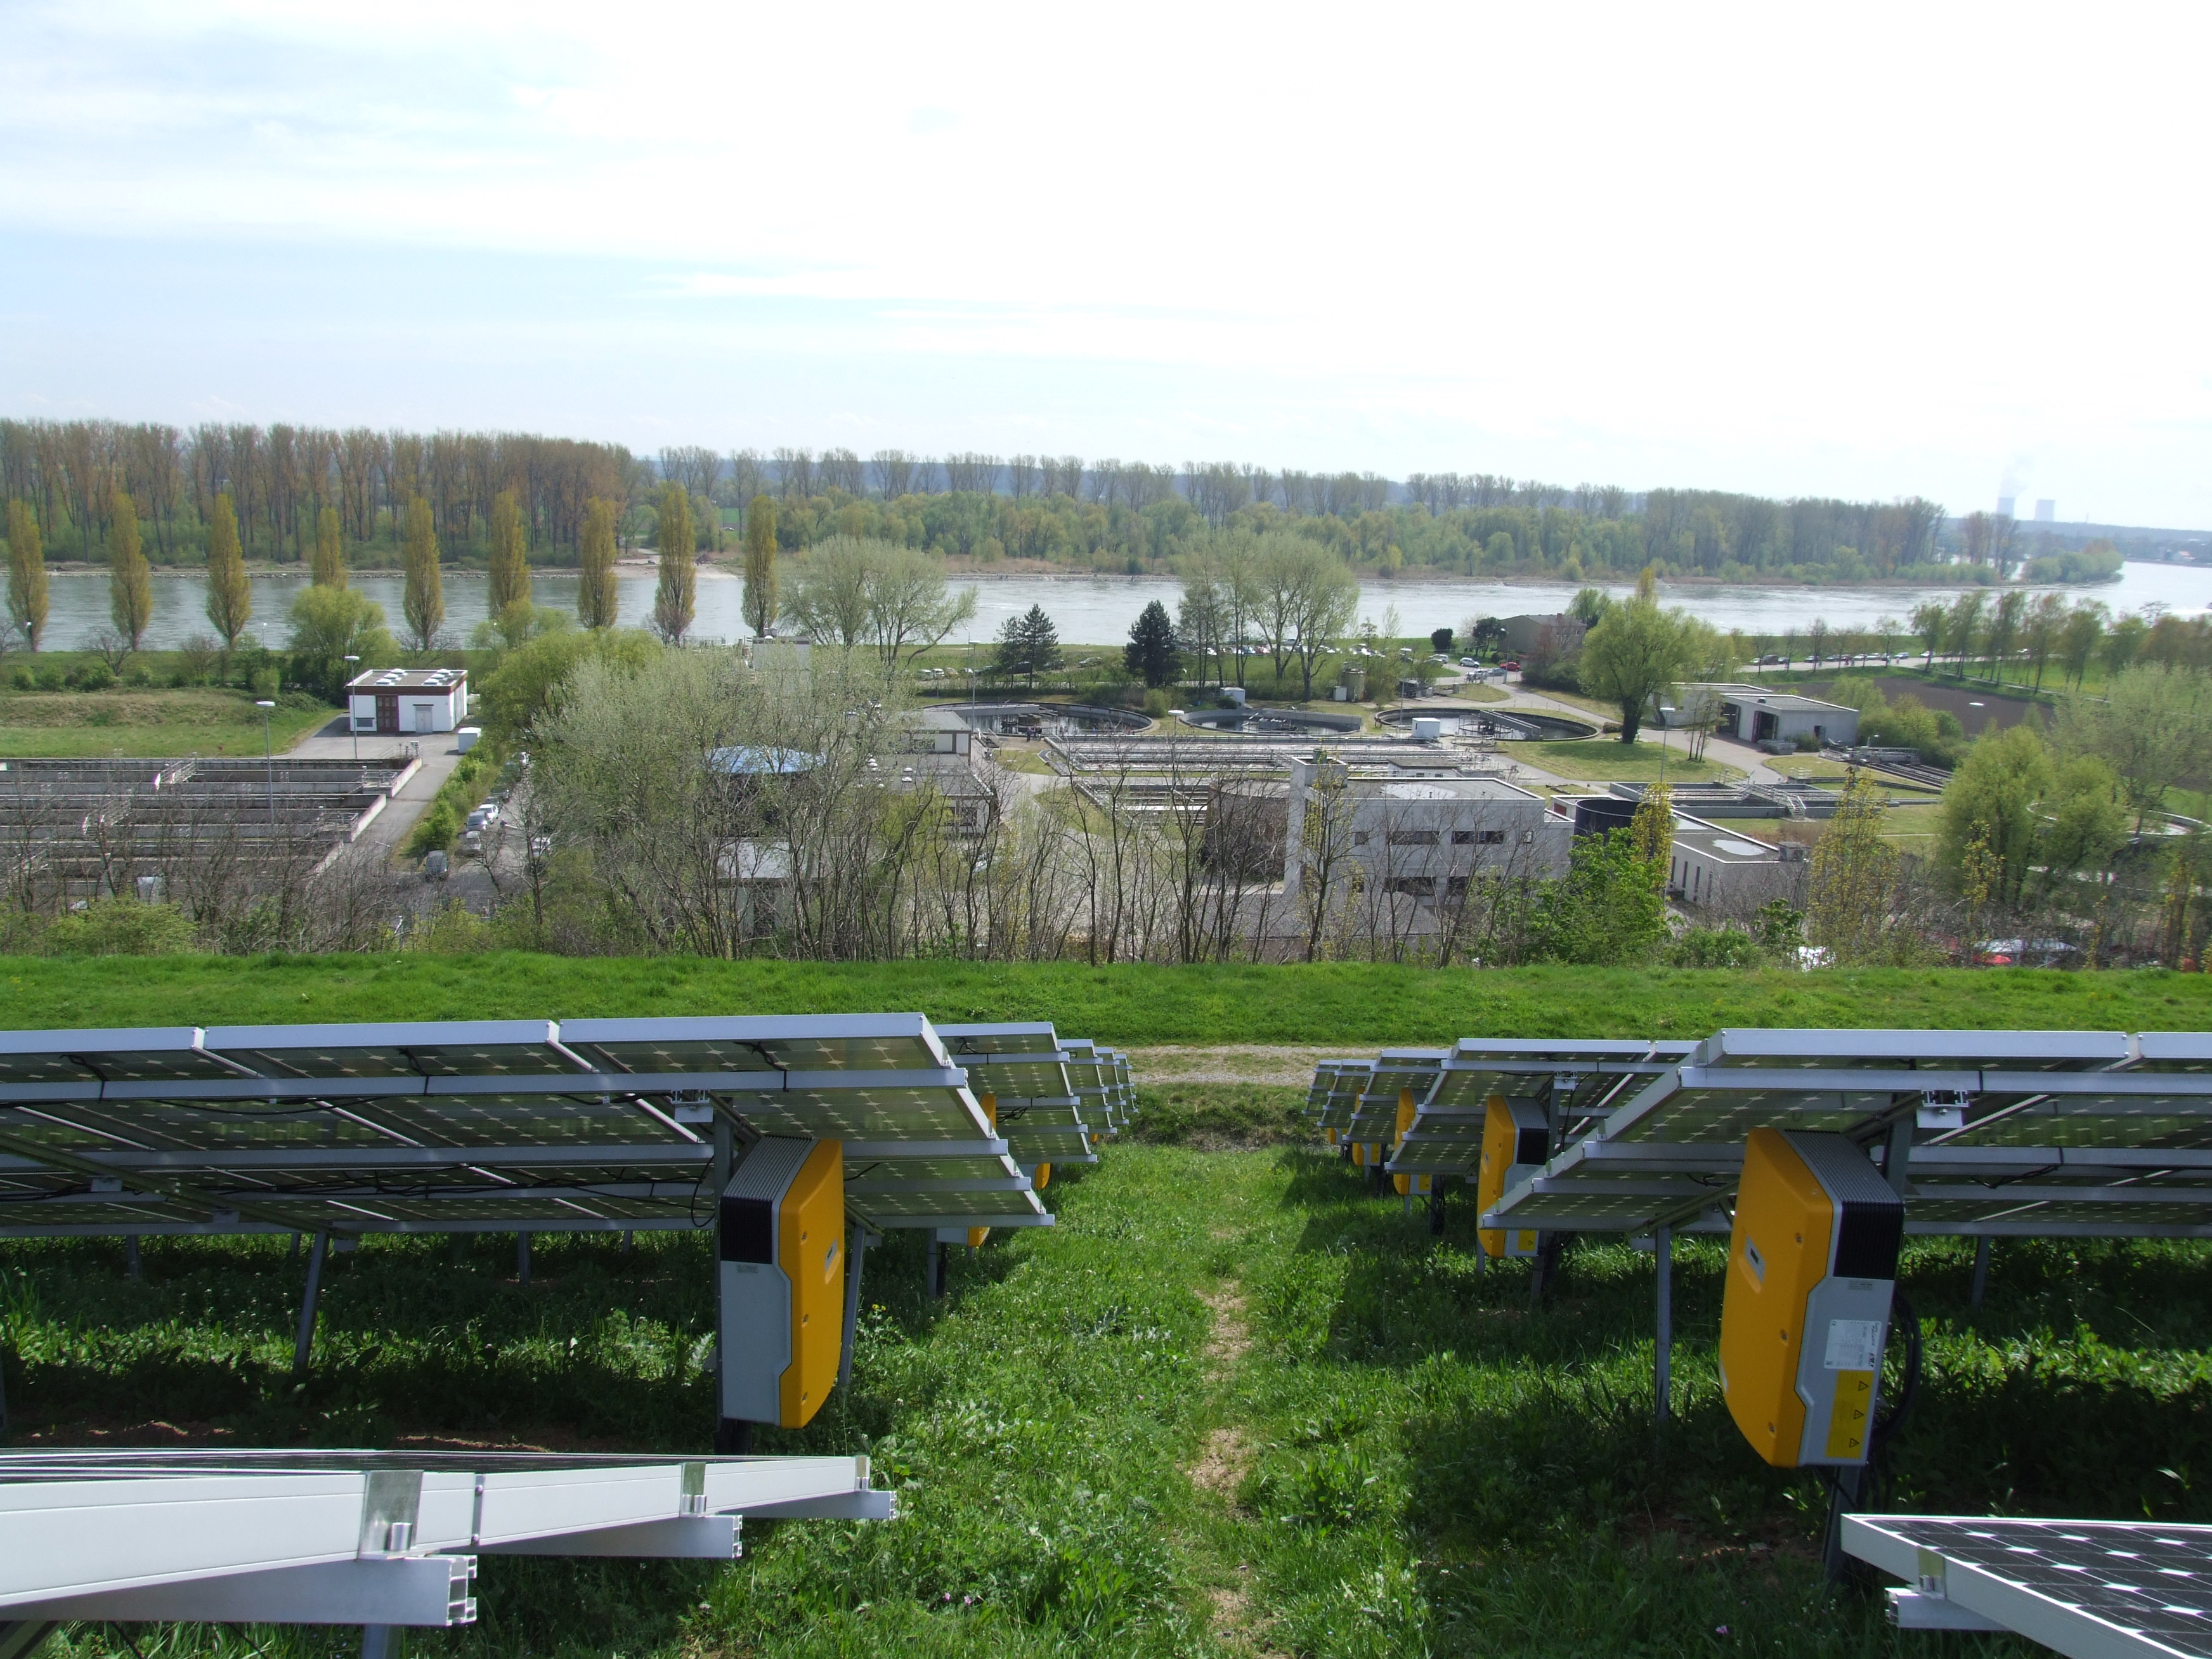
\includegraphics[scale=0.05]{fig/lec01/solar_inverter.jpg}
			\caption{A solar PV plant in  (source: \href{https://commons.wikimedia.org/wiki/File:Müllberg_Speyer_-_6_-_Rückseite_der_östlichen_Solarpanele.JPG}{Wikimedia Commons}, Claus Ableiter,\href{https://creativecommons.org/licenses/by-sa/3.0}{CC BY-SA 3.0})}
		\end{subfigure}
		\begin{subfigure}[t]{0.4\textwidth}
			\centering
			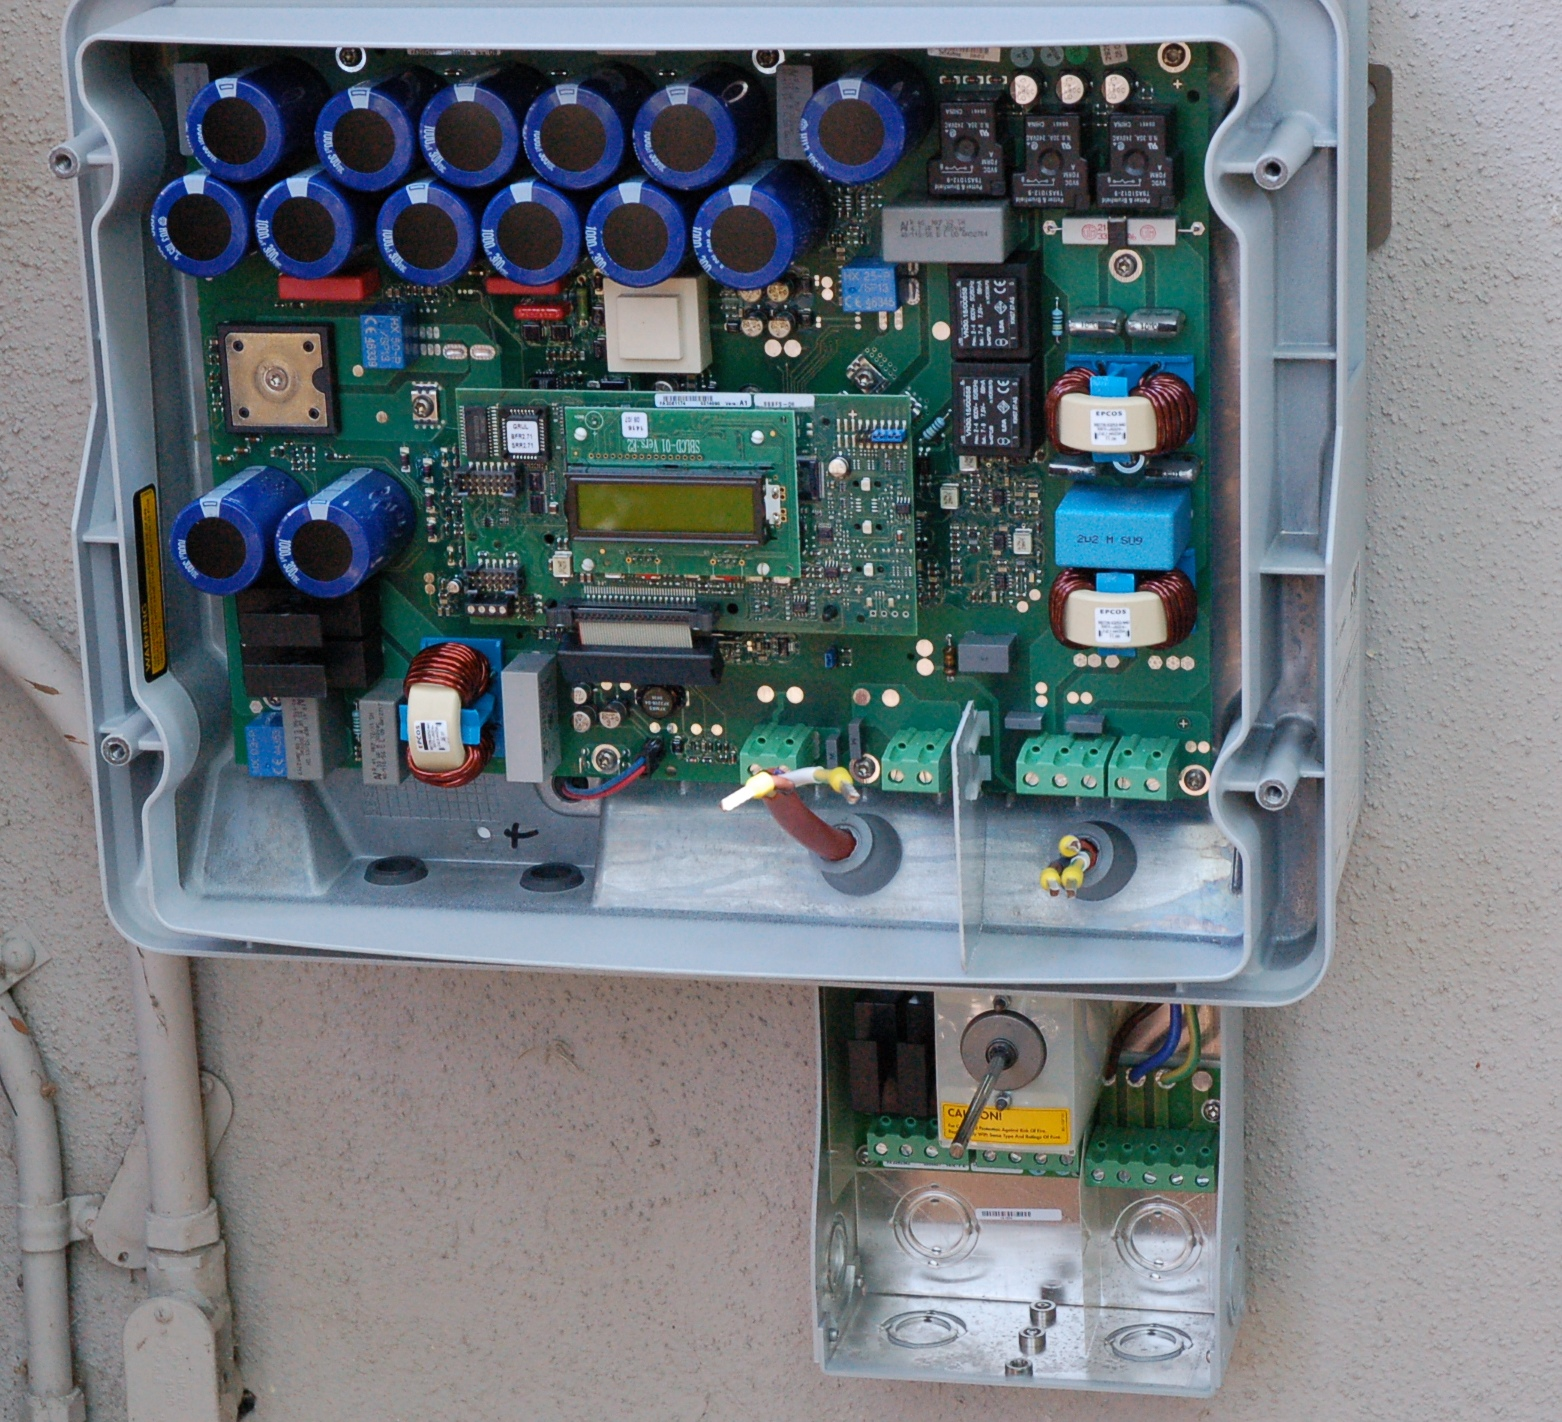
\includegraphics[scale=0.1]{fig/lec01/solar_inverter_open.jpg}
			\caption{Internal view of a solar inverter (source: \href{https://commons.wikimedia.org/wiki/File:Sunny_Boy_3000.jpg}{Wikimedia Commons}, Russell Neches, \href{https://creativecommons.org/licenses/by/2.0/}{CC BY 2.0})}
		\end{subfigure}
	\end{figure}
\end{frame}

%%%%%%%%%%%%%%%%%%%%%%%%%%%%%%%%%%%%%%%%%%%%%%%%%%%%%%%%%%%%%
%% Why are electric machines and drives important ? %%
%%%%%%%%%%%%%%%%%%%%%%%%%%%%%%%%%%%%%%%%%%%%%%%%%%%%%%%%%%%%%
\begin{frame}
	\frametitle{Why is knowledge about power electroics devices is important?}
	\begin{varblock}{Power Electronics more relevant than ever}
		Knowledge of power electronics devices is crucial for designing efficient systems that convert, control, and deliver electrical energy. It enables innovation in EVs, renewable energy, robotics, and industrial automation by optimizing performance, minimizing losses, and ensuring reliable operation. 
	\end{varblock}
	\begin{varblock}{Power electronics is the key to efficiency and sustainability}<2->
		Power electronic systems handle and convert more than 70\% of global electricity across industries such as transportation, energy, and automation (source: \href{https://www.hitachienergy.com/news-and-events/perspectives/2021/08/power-electronics-revolutionizing-the-world-s-future-energy-systems}{International Energy Agency}). With rising demands for electrification, advancing device efficiency and reliability is critical to minimizing energy losses, improving system performance, and enabling sustainable technologies across the globe.
	\end{varblock}
\end{frame}

%%%%%%%%%%%%%%%%%%%%%%%%%%%%%%%%%%%%%%%%%%%%%%%%%%%%%%%%%%%%%
%% Breakdown of an inductor %%
%%%%%%%%%%%%%%%%%%%%%%%%%%%%%%%%%%%%%%%%%%%%%%%%%%%%%%%%%%%%%
\begin{frame}
	\frametitle{Looking inside to define objectives!}
	%\vspace{-1cm}
	\begin{figure}
		\centering
		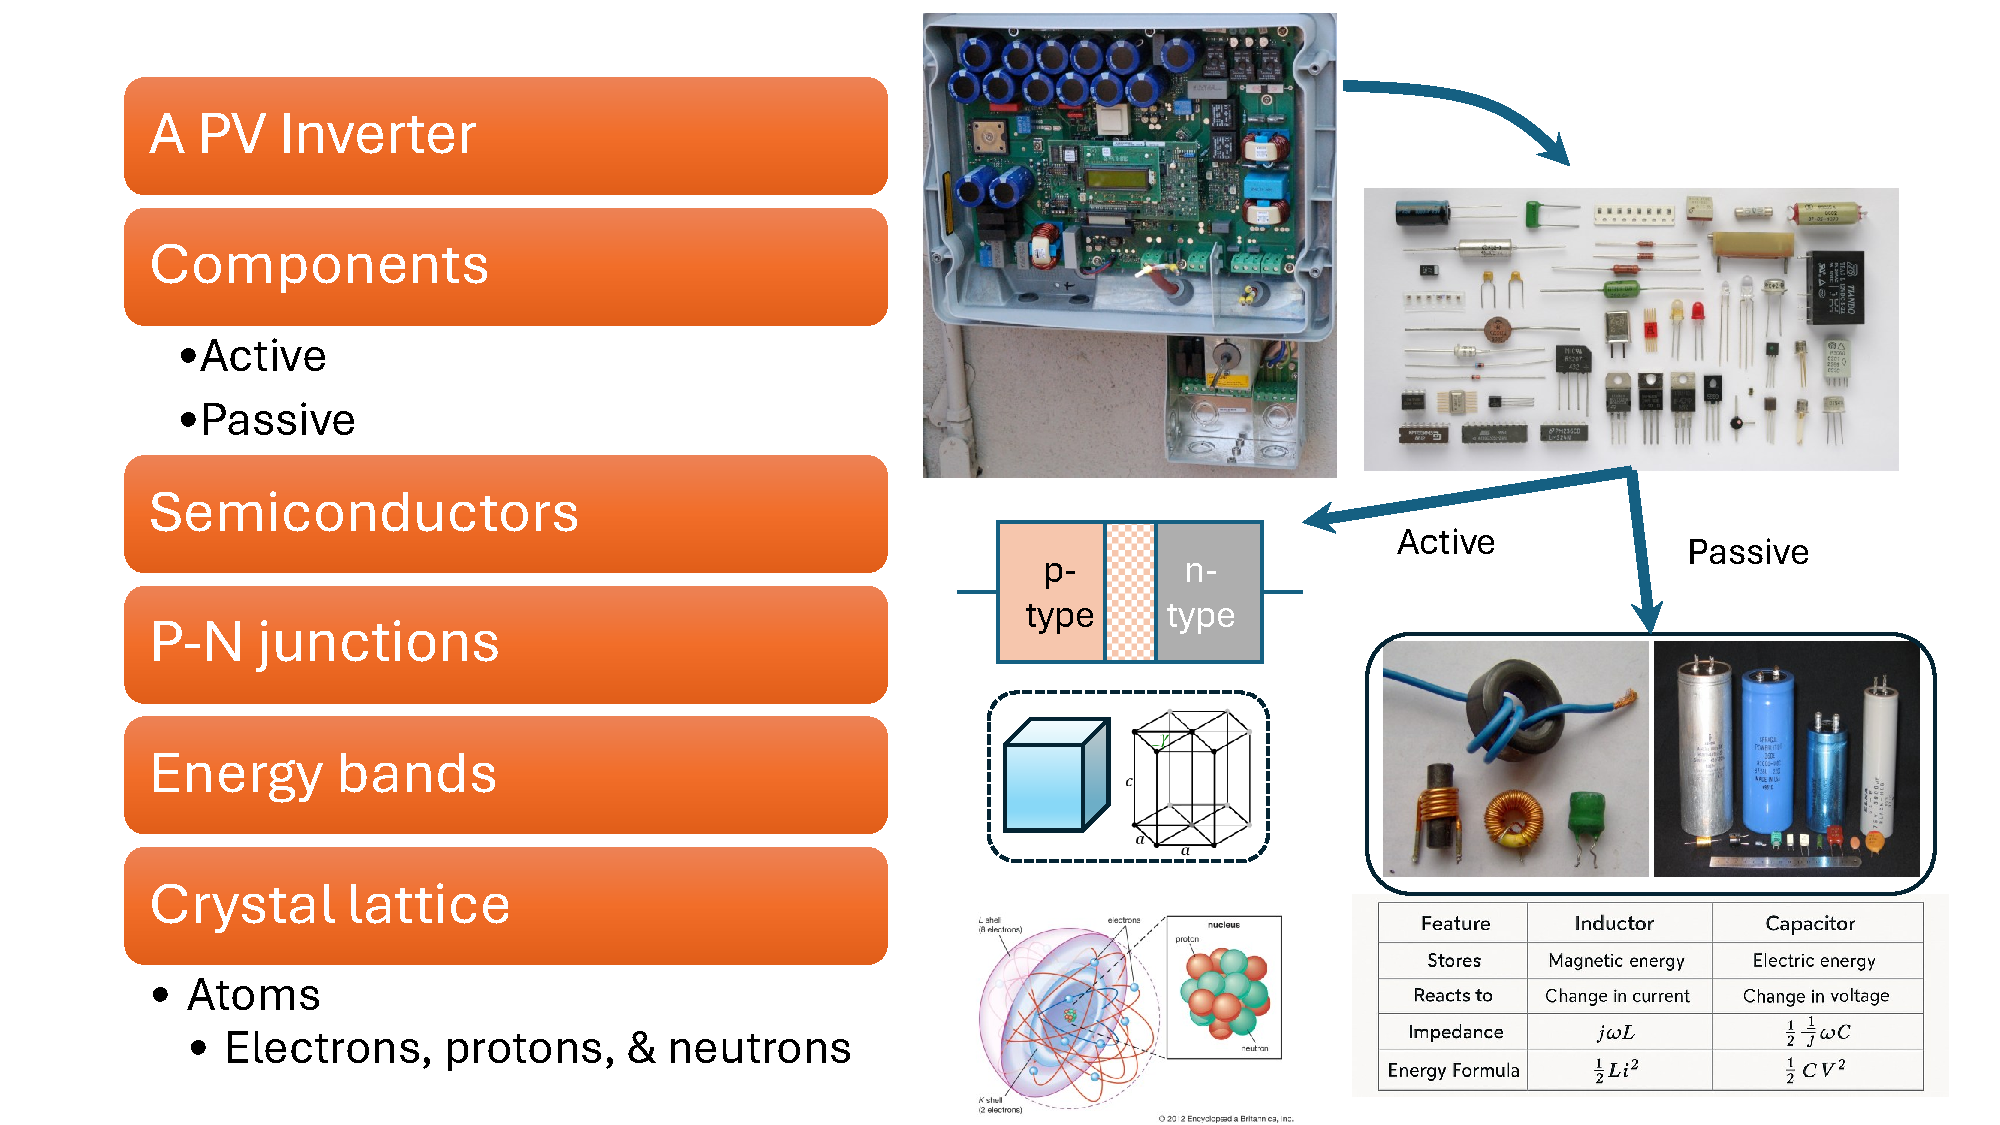
\includegraphics[scale=0.35]{fig/lec01/Flow_of_components.pdf}
		\caption{Definition of course and need (source: PV inverter, components, inductors, and capacitors \href{https://commons.wikimedia.org/wiki/Main_Page}{Wikimedia Commons}, multiple sources, public domain)}
	\end{figure}
\end{frame}

%%%%%%%%%%%%%%%%%%%%%%%%%%%%%%%%%%%%%%%%%%%%%%%%%%%%%%%%%%%%%
%% Learning objectives %%
%%%%%%%%%%%%%%%%%%%%%%%%%%%%%%%%%%%%%%%%%%%%%%%%%%%%%%%%%%%%%
\begin{frame}
	\frametitle{Learning objectives}
	\begin{itemize}
		\item Understand and explain the role of power electronics in modern energy systems, electrification, and sustainable technologies. 
		\item Understand the working principles of each device and components in power electronics.
		\item Analyze the physics of semiconductor materials and devices, including band theory, carrier transport, junction behavior, and breakdown mechanisms.
		\item Differentiate and evaluate the characteristics, structures, and operation principles of power semiconductor devices.
		\item Interpret and model switching characteristics, conduction behavior, and thermal limitations of conventional and wide-bandgap power devices (Si, SiC, GaN).
		\item Select and model active and passive components such as capacitors, inductors, transformers, and filters with consideration of frequency, losses, and application context.
		\item Have fun learning about power electronics devices and components.
	\end{itemize}
\end{frame}

%%%%%%%%%%%%%%%%%%%%%%%%%%%%%%%%%%%%%%%%%%%%%%%%%%%%%%%%%%%%%
%% Necessary prior knowledge %%
%%%%%%%%%%%%%%%%%%%%%%%%%%%%%%%%%%%%%%%%%%%%%%%%%%%%%%%%%%%%%
\begin{frame}
	\frametitle{Necessary prior knowledge for this course}
	You should have a basic understanding of the following topics:
	\begin{itemize}
		\item Basic electrical engineering knowledge (e.g., Ohm's law, Kirchhoff's laws, etc.)
		\item Basic understanding of physics in electronics
		\item Algebra and complex numbers
		\item Basic signal theory knowledge (e.g., Fourier series, Laplace transform)
		\item No advanced knowledge of semiconductors or programming is needed — this course builds those concepts from scratch and applies them to real systems.
	\end{itemize}
	\vspace{0.5cm}
	\onslide<2->What we will \underline{not} cover, but you do not need to know (covered in separate courses):
	\begin{itemize}
		\item Power converter circuits and topologies.
		\item Power electronics in depth involving analysis and controller design. 
	\end{itemize}
\end{frame}

%%%%%%%%%%%%%%%%%%%%%%%%%%%%%%%%%%%%%%%%%%%%%%%%%%%%%%%%%%%%%
%% Recommended reading %%
%%%%%%%%%%%%%%%%%%%%%%%%%%%%%%%%%%%%%%%%%%%%%%%%%%%%%%%%%%%%%
\begin{frame}
	\frametitle{Recommended reading}
	\begin{itemize}
		\item Baliga, B. Jayant. Fundamentals of power semiconductor devices. Springer Science \& Business Media, 2010.
		\item Lutz, Josef, Heinrich Schlangenotto, Uwe Scheuermann, and Rik De Doncker. "Semiconductor power devices." Physics, characteristics, reliability 2 (2011).
		\item Baliga, B. Jayant, ed. Wide Bandgap Semiconductor Power Devices: Materials, Physics, Design, and Applications. Woodhead Publishing, 2018.
		\item K. Niayesh, M. Runde, "Power Switching Components Theory, Applications and Future Trends", 1. Ed., Springer, 2018.
	\end{itemize}
\end{frame}